\documentclass[11pt, oneside]{article}   	% use "amsart" instead of "article" for AMSLaTeX format
\usepackage{geometry}                		% See geometry.pdf to learn the layout options. There are lots.
\geometry{letterpaper}                   		% ... or a4paper or a5paper or ... 
%\geometry{landscape}                		% Activate for for rotated page geometry
%\usepackage[parfill]{parskip}    		% Activate to begin paragraphs with an empty line rather than an indent
\usepackage{graphicx}				% Use pdf, png, jpg, or eps� with pdflatex; use eps in DVI mode
								% TeX will automatically convert eps --> pdf in pdflatex		
\usepackage{amssymb}

\title{Integration}
%\author{The Author}
\date{}							% Activate to display a given date or no date
\graphicspath{{/Users/telliott_admin/Dropbox/Tex/png/}}

\begin{document}
\maketitle
%\section{}
%\subsection{}
\large
\begin{center}
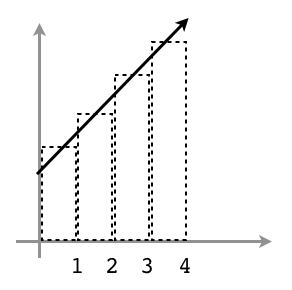
\includegraphics [scale=0.5] {rects.png}
\end{center}
The topic of integration is often introduced using area, although as we gain understanding we will see that it's much more versatile than that.  In the figure above, our goal is to compute the area above the $x$-axis and below the graph of $f(x)$.  Our region is bounded by the two vertical lines $x=0$ and $x=4$ (more generally, it will be $x=a$ and $x=b$).

The general approach is to think of a bunch of little boxes, each with height equal to the value of $f(x)$ somewhere in the range of $x$ for the box.  We add up the areas of these boxes (that is, the value of $f(x)$ for each box, times the width which equals one here), and that's our estimate for the area.  In the figure, I've drawn the boxes with heights 

\[ f(0.5) + f(1.5) + f(2.5) + f(3.5) \]

However, we could just as well do 

\[ f(0) + f(1) + f(2) + f(3)  \]

or

\[ f(1) + f(2) + f(3) + f(4) \]

In the case where we start at $f(0)$, at the left side of the range of $x$, we would clearly end up with an under-estimate, while ending at $f(4)$ will yield an over-estimate.  The approach shown is more somewhat more accurate.

In other words, the question is whether the boxes should touch the curve $f(x)$ at the left, in the middle, at the right, or somewhere else.  In the end, it will turn out that \emph{this doesn't matter}.  The reason is that we will imagine shrinking the width of the boxes so they become almost infinitely thin (and of course, increasing their number accordingly in the process).

Also, I used a straight line in this figure, but the function could be anything.  As our second example, we will take the function $f(x) = x^2$.  For the region, we choose $0 < x < 1$.  We will construct $n$ rectangles that reach up to the correct value for $f(x)$ at that point.  The width of each rectangle is $1/n$.  

The height depends on the location of the box.  The first rectangle $R_1$ lies at $x=1/n$ and has height:
\[ h_1 = (\frac{1}{n})^2 \]

Note that this amounts to using the right-hand edge of the box to compute $f(x)$.
For $R_k$ we have $x=k/n$ and height
\[ h_k = (\frac{k}{n})^2 \]
For each box we have to multiply width $\times$ height.  The width is $1/n$ for each.  Adding up the areas for all the boxes we have that the total area is
\[ A = \ [ \ \frac{1}{n} \ ( \frac{1}{n})^2 + \frac{1}{n} \ (\frac{2}{n})^2 + \cdots + \frac{1}{n} \ (\frac{n}{n})^2 \ ] \]
\[ A = \frac{1}{n^3} \ [1^2 + 2^2 + \cdots + n^2 ] \]
There is a formula for the sum of the squares of the first $n$ integers, we just plug it in and get
\[ A = \frac{1}{n^3} \ \frac{n(n+1)(2n+1)}{6} \]
\[ A = (\frac{1}{6}) (\frac{n}{n}) (\frac{n+1}{n}) (\frac{2n+1}{n}) \]
The ratio $n/n$ is equal to $1$.  In the limit as $n$ gets very large, the ratio $(n+1)/n$ approaches $1$, and the ratio $(2n+1)/n$ approaches $2$.  So we have $2/6$ which equals $1/3$.

It is worth pointing out that this is exactly where the factor of $1/3$ comes from in the famous volume formula for a cone and pyramid, as well as the factor of $2/3$ in the volume of a hemisphere (by subtracting $1 - 1/3$).

\subsection*{}

If $x=b$, then the width of each piece would be $b/n$ and the heights would be $(b/n)^2$ and so the whole area would be multiplied by $b^3$.

Also notice that if we didn't want to start at $0$ but at some point $x=a$, then what we would do is to calculate two areas, one from $0$ to $a$ and one from $0$ to $b$, and the area from $a$ to $b$ is obtained by subtraction.

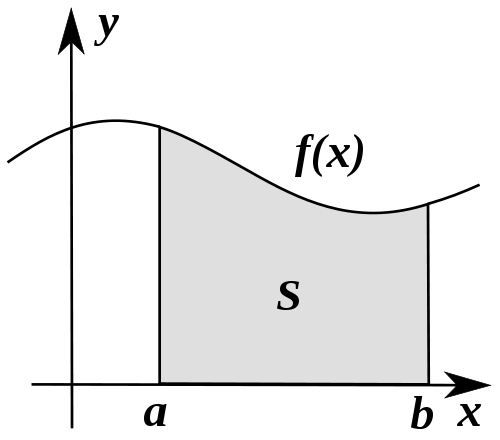
\includegraphics [scale=0.3] {int_area.png}

The transition to calculus comes by looking at the area as a function $A(x)$.  Suppose we have calculated some area $A(b)$, the area between $x=0$ and $x=b$.

Now we move $x$ just a little bit ($h$) to the right of $b$.  By how much will the area change?  The rate of change of the area with respect to a small change in $x$ is just $f(x)$.  But the rate of change of the area with respect to a small change in $x$ is, by definition $d/dx$ of A(x)

\[ A'(x) = \frac{d}{dx} A(x) = \frac{dA}{dx} = f(x) \]
We can put the $dx$ on the other side and then add up all the little pieces of area

\[ A(x) = \int dA = \int f(x) \ dx \]

If we are given $f(x)$ and asked for the area function, we need to find a function whose derivative equals $f(x)$.

In the case of the first example above, we had $f(x) = x^2$.  We know a function that gives this as the derivative, it is $(1/3)x^3$.  We have
\[ A(x) = \frac{1}{3}x^3 \]
\[ A(a) = \frac{1}{3}a^3 \]
Exactly as we found before.
\end{document}  